
\usetikzlibrary{arrows.meta} % For double arrows

\chapter{BitTorrent Protocol}

BitTorrent is a peer-to-peer file sharing protocol that allows nodes to 
distribute data in a de-centralized fashion. The tracker is the central server
that knows all the members in the cluster. A node coming online learns about its
peers by talking to the tracker. Once a node learned about the peer nodes, the
node can initiate data exchange with its peers directly.

\pagebreak

The following is a BitTorrent cluster with five nodes:

\begin{center}
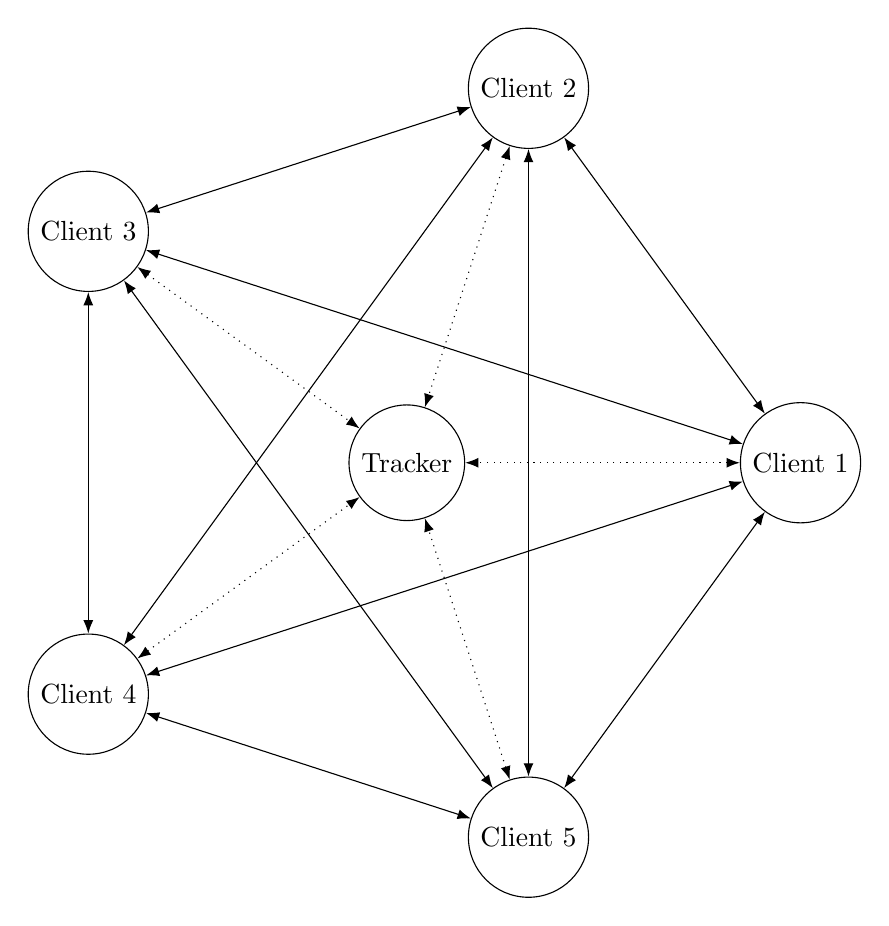
\begin{tikzpicture}
    % Draw 5 "client" nodes in a bigger circle, labeled from 1 to 5
    \foreach \angle/\label in {0/1, 72/2, 144/3, 216/4, 288/5} {
        \node[draw, circle] (client\angle) at (\angle:5cm) {Client \label}; % Increased radius to 5cm
    }

    % Draw the "tracker" node in the center
    \node[draw, circle] (tracker) at (0,0) {Tracker};

    % Draw double-ended dotted lines from each client to the tracker
    \foreach \angle in {0, 72, 144, 216, 288} {
        \draw[Latex-Latex, dotted] (client\angle) -- (tracker);
    }

    % Draw single-line, double-ended arrows between all client nodes
    \foreach \source in {0, 72, 144, 216, 288} {
        \foreach \target in {72, 144, 216, 288, 0} {
            \ifnum\source<\target % Avoid duplicate and self-loops
                \draw[Latex-Latex] (client\source) -- (client\target);
            \fi
        }
    }
\end{tikzpicture}
\end{center}

\section{Design}

\section{Spec}

\begin{tla}
    
\end{tla}